\chapter{Miért}

\section{Kétség és Hit}

\keywords{kényszeres gondolatok, nézetek irányba igazítása, váratlan változások}

\noindent Előfordul, hogy azért érdekel minket a meditáció, hogy meg
tudjunk birkózni egy felkavaró vagy fájdalmas tapasztalattal. Tudjuk,
hogy `valami nincs rendjén', és nem tudjuk lerázni az érzést. Vagy lehet
ez a veszteség fájdalma, ami olyan zavar érzését kelti, amiben látszólag
semminek sincs értelme: az ilyen érzések egyre csak visszatérnek, nem
engedik magukat figyelmen kívül hagyni. Válaszok helyett, csak a
gondolataink járnak körbe-körbe: `Miért kell ennek így lennie? Mit
kellene tegyek, és miért? Mi értelme ennek?'

Még az ilyen zavart állapotban is, pusztán elismerni magunknak a belső
káosz állapotát is már elkezd irányt és rendet teremteni.

Ahhoz hasonlít ez, mintha olyan úton vezetnénk, ami tele van szórva
szeméttel. Lelassítani és körül nézni máris sokkal jobb, mint vaknak
lenni a veszélyes hulladékra. Tele van a fejünk gondolatokkal, de
közöttük kevés mutat megbízható irányba, így jobb, ha megvizsgáljuk
őket. Korábban volt egy elképzelésünk, hogy a dolgok hogy állnak a
világunkban, de ezek megváltoztak olyan módon, amire nem számítottunk.
Nem a dolgok hibája, nem a mi hibánk, de a váratlan változás megzavaró,
és nézetünket igazítanunk kell.

Az állandótlanság kirántja a lábunk alól a szőnyeget, de egyúttal át is
alakítja az értékeinket, azokat a jellemzőket, amiket keresünk és
értékesnek tartunk a tapasztalatainkban. Ha nem értjük a változást, az
zavart okoz, amit kétség követ. Talán tudjuk, mit \emph{kellene
tegyünk}, de a kétség és jelentés nélküliség érzetében elakadunk, és el
sem tudjuk kezdeni.

\keywords{jelentés, vizsgálni mit hiszek, hit mint üzemanyag}

Miért kelsz fel reggel, hogy tegyél bármit is? Miért számít egyáltalán?
Ha folytatom a `miért' kérdéseket, és így beleások a felépített énem
rétegeibe, az első réteg a megszokott rutint tárja fel, `mert ezt
csináltam tegnap is.' Ez alatt, a válaszokat olyan történek formálják,
amiket én mondok magamnak arról a világról, amiben élek. Ez alatt, van
valamilyen érvelés, filozófia és absztrakt ötletek. Ez alatt, kezdek
kétségbeesetten kapaszkodni valami szilárd dologba, és elkezdem
emlékekkel és tapasztalatokkal védeni az elképzeléseimet (`mert amikor
így megy így jártam\ldots{}'), vagy híres személyekre hivatkozok (`mert
ez és az a tanító azt mondta\ldots{}').

Ez alatt, fel kell adjam és bevallanom, hogy a dolog hit és személyes
meggyőződés kérdése. Amit teszek, egyszerűen az, amit eldöntök ott és
akkor. A végén ott állok, hogy \emph{nem tudom, de úgy hiszem}, hogy azt
tenni értelmes dolog.

A hit nem egy rögzített jellemző az elmében, megvan a kapacitásunk, hogy
megválasszuk a hitelt érdemlő állításokat amiket úgy látunk, hogy
nagyobb megismerés és boldogság felé irányítanak minket.
Alátámaszthatjuk, vagy elhagyhatjuk a hitet azzal, hogy gyakorlatban
alkalmazzuk és figyelünk az eredményekre.

Ellenőrizhetem, felülvizsgálhatom és frissíthetem \emph{mit hiszek}
arról, hogy minek van értelme, de amíg a tapasztalatom nem igazolja azt,
az érvelésemet a hitnek kell alátámasztania. Különben nem fogok
erőfeszítést tenni semmilyen irányba, és az életemet vak szokások és
külső nyomások fogja uralni.

A hit az elhatározás és energia erényeinek üzemanyaga. Később, a hitet
megerősíti az, hogy magunkon érezzük a gyakorlás eredményeit, de
üzemanyag nélkül, az autónk el sem indul.

\keywords{hit mint a tett kiváltó oka, bizalom a tanítóban}

A hit okot teremt a tettre. Hit nélkül, nem teszem meg az adott dolgot.
A buddhista látásmódban két alapvető hittétel van:

\begin{enumerate}
\item
  Egy jelenség megtörténik, ha az elégséges feltételek megvannak hozzá,
  és nem történik meg, vagy megszűnik, ha az elégséges feltételek
  hiányoznak.\footnote{\href{https://www.dhammatalks.org/suttas/SN/SN12_61.html}{SN
    12.61}, Tanulatlan}
\item
  A Buddha teljesen megértette az igazságot arról, ahogy a dolgok
  vannak, és így megszabadította magát a mohóságtól, gyűlölettől és
  zavarodottságtól. Emiatt kiváló tanítója a gyakorlás útjának.
\end{enumerate}

A Buddha arra adott utasítást, hogy mindenkinek magának kell
rákérdeznie, töprengenie, és megvizsgálnia azt, hogyan vannak valójában
a dolgok, hogy megértse azt. De mégis, hogyan fogjunk hozzá? A tanítóban
való hit nélkül, el vagyunk veszve a személyes véleményeink
kuszaságában, és nem valószínű, hogy hallgatni fogunk másra és tanulni
valami újat. A hagyomány erre a kapcsolatra emlékeztet minket, amikor
egy Dhamma beszéd előtt, a \emph{namo tassa} sorait kántáljuk háromszor.

\begin{quote}
\emph{Namo tassa bhagavato arahato sammā-sambuddhassa}

Tisztelet a méltóságos Magasztosnak, a saját erejéből tökéletesen
megvilágosodottnak.
\end{quote}

\keywords{kétség, sivatagban bolyongani, a ragaszkodás korlátokat teremt}

A Buddha ahhoz hasonlította a kétséget, mintha egy sivatagban
bolyonganánk víz nélkül.\footnote{\href{https://suttacentral.net/dn2}{DN
  2}, A Szerzetesi Élet Gyümölcsei} Minden más másodlagos, csak arra
tudunk gondolni, hogyan találjunk vizet és jussunk ki a sivatagból.

Vagy, hogyan tompítsuk el az elmét és egyáltalán ne gondoljunk semmire,
`álomba ringatni magunkat a trivialitással'\footnote{Søren Kierkegaard,
  `A halálos betegség'}, hogy mindent úgy folytathassunk mint eddig. A
kétség miatt nem világos, hogyan szabadulhatunk ebből a helyzetből, de
kezdhetjük azzal, hogy elismerjük magunkban a törekvést, hogy jól
legyünk és boldog életet éljünk.

Emberi természetes képességünk, hogy túljussunk a zavaron és hosszú távú
boldogságot fejlesszünk az életünkben. A hosszú távú szemléletnek magába
kell foglalnia a helyzetünk változását, a veszteséget és tragédiát. A
stabil boldogságnak olyan szemléletre kell alapulnia, amely magába építi
az állandótlanságot.

A szuttákban, a kétség szerepel az Öt Akadály listáján is, és Tíz Béklyó
első három eleme között is, melyek eltakarják a Négy Nemes Igazság
megértését. Mikor személyesen érint, nincs kétség, hogy a kétség
szenvedéshez vezet. Az ábrák \ref{fig-leading-to-suffering} és
\ref{fig-leading-to-cessation} illusztrálják hogyan kerülünk ebbe a
káoszba, és hogyan tudunk kijutni belőle.

Mint akadály, a kétség megállítja a Helyes Erőfeszítést, és megállítja
az elme fejlesztését. Mint béklyó, arra késztet, hogy fix
bizonyosságokat keressünk, és így még szorosabban köt minket az
elképzeléseinkhez arról, kik vagyunk.

Szeretjük a javaslatot, hogy fejlesszük az elménket, de kezdetben azt
gondoljuk, ez azt jelenti, hogy megerősítsük kik és mik vagyunk, többet
szerezzünk abból amire szükségünk van, vagy megváltoztassunk magunkat és
valami mássá váljunk.

`Ki vagyok? Mi vagyok? Mit kellene tegyek? Ez itt a megfelelő dolog,
vagy egy másik?' Ez a fajta gondolkodás egy csapda, körbe-körbe jár kiút
nélkül. Mindezek a kérdések ahhoz kötődnek, hogy valamilyen
ön-azonossághoz ragaszkodunk, ami újra kétséget fog magával hozni. Amíg
nem vesszük észre mi történik, benne ragadunk a körforgásban.

Még amikor sikeresek is vagyunk, annak a végén, hogy valamivé váltunk,
az meg fog változni saját természeténél fogva, és azt találjuk, hogy az
új azonosságunk is hiábavaló, üres, valódi érték nélküli, akár csak a
korábbi elképzelésünk magunkról.

\enlargethispage*{\baselineskip}

Ahhoz ragaszkodni amiről azt gondoljuk, mi vagyunk, félni az
elengedéstől: ez az akadály. Ez hozza létre éppen azt a korlátot, aminek
frusztráltan neki ütközünk. A szabadságot az elengedésen keresztül
megérteni nem megy nekünk egykönnyen.

\cleartoverso
\figurepagelayout

\begin{figure}[h]
\vspace*{-10mm}%
\caption{Szenvedéshez Vezet}\label{fig-leading-to-suffering}

\centering

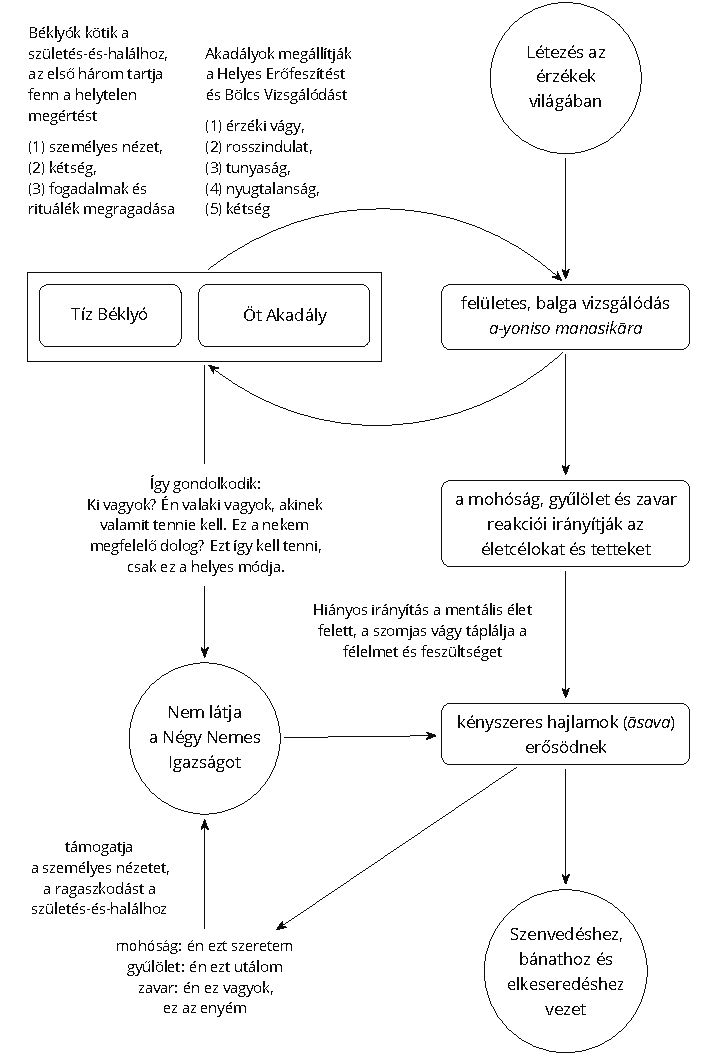
\includegraphics[width=\linewidth]{./manuscript/tex/diagrams/leading-to-suffering-hu.pdf}

\end{figure}

\clearpage

\begin{figure}[h]
\vspace*{-10mm}%
\caption{Megszűnéshez Vezet}\label{fig-leading-to-cessation}

\centering

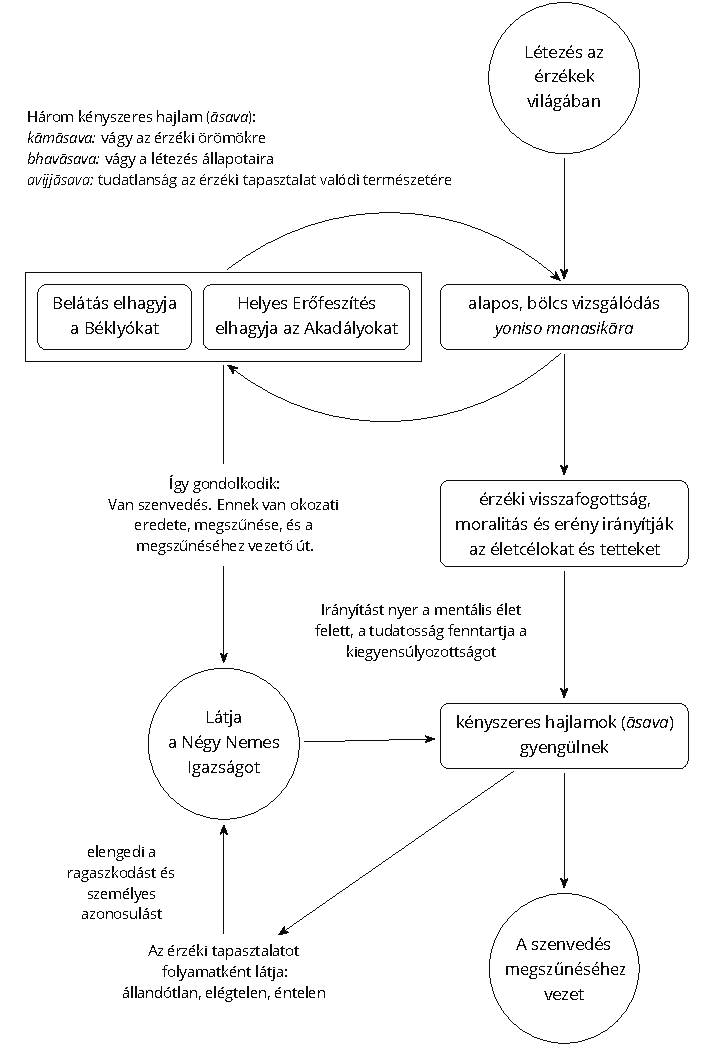
\includegraphics[width=\linewidth]{./manuscript/tex/diagrams/leading-to-cessation-hu.pdf}

\end{figure}

\clearpage
\normalpagelayout

\section{Helyes Nézet}

\keywords{visszatérni a kezdethez, gondolatok megfigyelése}

\noindent Térjünk vissza a légzéshez és folytassuk a meditáció
gyakorlását. Kezdd a gyakorlat elejét az alapokkal, egyszerű lépésekkel
amik vissza terelik a figyelmet a jól ismert keretbe: be- és kilégzés, a
test és annak érzései. Figyeld amit tapasztalsz egy folyamatként, ami
állandó változáson keresztül az egyik érzésből a másikba alakul át.

Minden meditáció egy új kezdet, nem menthetjük el az előző alkalom
eredményeit, hogy most betöltsük a tudást. Ha úgy kezdjük, hogy azt
gondoljuk mi ezt már tudjuk, mondjuk, ha már évek óta gyakoroljuk ezt,
ez egy zárt hozzáálláshoz vezet, ami blokkolja a korábbi megértésünket
is. A múltból származó tapasztalatunk csak úgy értékes, ha a jelenre
vonatkozóan alkalmazzuk. A változó jelen a megértést megújítja és
frissen tartja.

`Ennek a gondolatnak, ennek az érzésnek volt kezdete, most változik, meg
fog szűnni és vége lesz. Meg tudom várni és észre venni azt az
elmúlást?' A közvetlen tapasztalatot így szemlélve, az elme feladja a
vágyat és félelmet az adott állapotokkal kapcsolatban, és megérti őket
mint természetes folyamatok részeit. Nem azt bizonygatjuk magunkban mit
gondolunk az elméről, hanem mintha egy lépést hátralépve szemlélnénk,
éberen tapasztaljuk azt, ahogy van.

Ez a szemlélődés vissza állítja a Helyes Nézetet, mintha egy fordítva, a
fején álló virág vázát valaki újra egyenesen felállítana. Mikor ránézünk
értjük, hogy a vázának melyik része az alja és melyik a teteje.
Szomjasan kívánjuk és ragaszkodunk olyan tapasztalatokhoz, amik mindig
változni fognak, nem hangzik ez feszültségnek és szenvedésnek?
Szerencsére a hiba elkerülhető.

\keywords{korlátok körüli szabadság, lényeg, hála érzet, elárasztva a jó tanáccsal}

A Helyes Nézet megtalálja a teret és szabadságot az élet korlátai és
nyomásai körül. Eleinte talán nem látunk túl sok szabad teret, de a
lényeges dolgokat megvizsgálva észrevehetjük, hogy nincs szükségünk
mindenre amire gondolni tudunk. Megkérdezhetjük, `Megvan, amire
szükségem van erre az egy napra?'

Sorra vehetjük mit használunk a közvetlen környezetünkben -- ruha, étel,
szállás, gyógyszerek. Egyszer mi kapjuk valakitől, vagy engedik, hogy
használjuk, máskor mi adjuk másoknak. `Tudom mennyi elég a mai napra?'
Úgy érzem visszatér a nyugalom, mikor újra felidézem őket, még ha már
jól ismerem ezeket a tényeket.

Felidézve az egyszerű dolgokat, hogy megvan amire szükségünk van, hogy
jól éljük ezt a napot, a hozzáállásunk abban fejezi ki magát, hogy
megnyugvást és hálát érzünk az életért. Nem kell kérned ezt, és nem
tudod akarattal létrehozni. Teret kell adjunk neki a szemléletünkben, és
magától megjelenik.

Hova ez a nagy sietség? Egy egyszerű gyakorlat, hogy megállunk két
percre, nem keresni szórakoztatást és figyelemelterelést, egyszerűen
semmit nem tenni két percig. Figyelheted a lélegzetet, de ez is
választás kérdése. Nem elutasítani az unalmat, mint elme állapotot,
növeli az összpontosításunkat és energiánkat.

A probléma nem az, hogy nincs nem tudunk eleget. A könyvespolcok
túlcsordulnak a jó tanáccsal arról, `hogyan legyünk boldogok'. Ha csak
ez kell, akkor hol a hiba? Ha csak a jó tanácson múlna, már mindannyian
rég megvilágosodtunk volna. Halljuk és olvasunk arról, hogy mi minden jó
dolgot kellene tennünk, milyenféle embernek kellene lennünk: az egyik
könyv szerint legyünk kemények és félelem nélküliek, miközben a másik
szerint univerzális együttérzésre van szükségünk. A szenvedés egy külön
fajtája végigolvasni az egészet.

Vagy talán a \emph{Nibbánára} van szükségünk? Ez a helyes elképzelés? A
szó jelentése \emph{elhűlt, hűvös}, gondolhatunk egy tűzre, ami kialszik
és elhűl. A szomjas vágy, hogy `megszerezzük', csak több tüzelőanyagot
jelent a létesülés hőségéhez és tovább égéséhez.

De a \emph{Nibbána} a létesülésben égés kialvásának hűvössége, tehát
ilyen nem-létesüléssé kellene váljunk? A gondolkodó elme erre az mondja,
`\emph{Mi van?!}' És ez nem is rossz válasz: a Buddha tanítása arra
mutat rá, hogy a gondolkodás és létesülés nem elégséges eszközök ehhez.
Egy újabb állapot vagy gondolat, mikor magunkat látjuk benne, olyan
korlátozó lesz mint a korábbi. Nem abban áll a szabadságunk, hogy a
megfelelő dologgá válunk, hanem a felismerésben, hogy fel tudjuk adni a
kényszert, hogy a folyton valamivé válnunk kelljen.

\clearpage
\figurepagelayout

\begin{figure}[h]
\caption{Tapasztalat, Létesülés és a Haláltalan}\label{fig-experience-becoming-deathless}
\bigskip
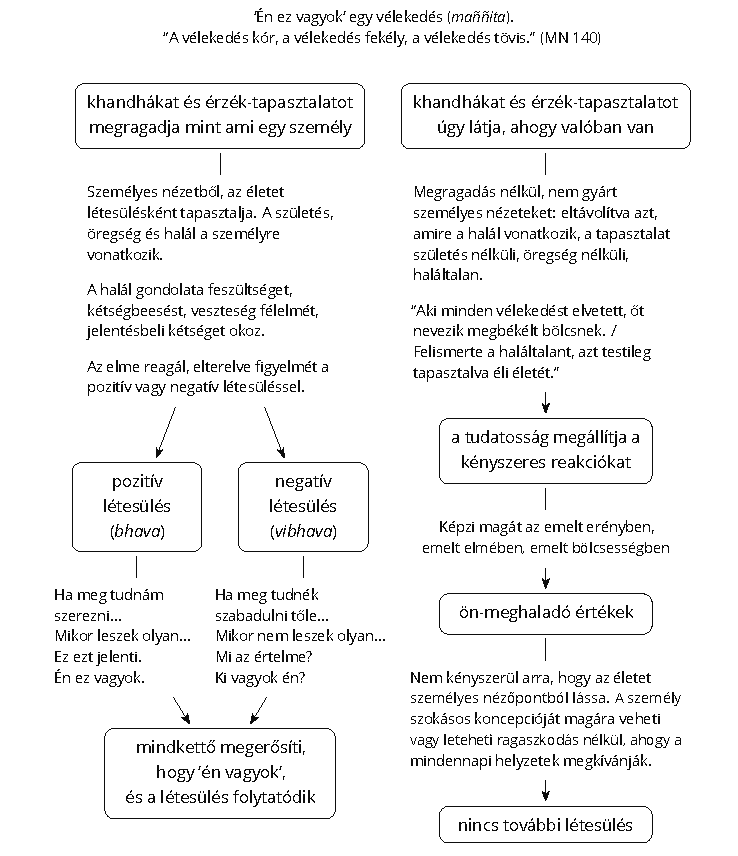
\includegraphics[width=\linewidth]{./manuscript/tex/diagrams/experience-becoming-deathless-hu.pdf}
\end{figure}

{\noindent\footnotesize
Lásd még: Chapter 10, Birth, Decay and Death in The Buddha's Teaching: It's Essential\\ Meaning by R. G. de S. Wettimuny
\par}

\clearpage
\normalpagelayout

\section{Új Szemmel}

\keywords{a tapasztalat felé fordulni, intellektuális tudás, az érzékek figyelése}

\noindent Egy kényszeres hajlamot helyes nézetté változtathatunk át, ha
megkérdezzük, `Hogyan tudom megérteni ezt a tapasztalatot?' Ez a kérdés
a nemes hozzáállás felé irányít minket, amit az Első Nemes Igazság
tartalmaz: `A szenvedést meg kell érteni.' Tedd félre a véleményeket,
melyek válaszként mutatkoznak, és folyton térj vissza ehhez a nyitott
hozzáálláshoz, ami ismeri a jelen pillanatot.

Az öröm és a bánat mind természetes folyamatok, de ha nem értjük őket,
az egyiket jutalomnak tekintjük, a másikat pedig büntetésnek. Úgy tűnik,
az élet sosem igazságos, és mindig úgy tűnik, hogy az irányításunkon
kívül esik.

Ahhoz, hogy megnyissuk a hozzáállásunkat a vizsgálódáshoz, legalább el
kell tudjuk képzelni a lehetőséget, hogy van itt valami amit meg tudunk
tanulni. Egy fordulóponthoz érkezünk, el tudjuk engedni, hogy biztosak
legyünk a véleményeinkben, és megállunk megvizsgálni magát a
tapasztalatot.

Vedd figyelembe, milyen szűk a szemléletünk, amikor azzal a gondolattal
kezdünk, hogy `Ezt már láttam, én ezt ismerem.' Lehet, hogy ez igaz, de
azt veszem észre, hogy amikor ezt az intellektuális információt próbálom
használni egy probléma megoldásához, a figyelmem csupán emlékek,
gondolatok és vélemények körül forog. Amíg magával ragad a múlt, a jelen
tapasztalat elkerüli a figyelmem.

A Buddha utasítása, hogy óvatosan alapozzuk meg a szándékunkat a
meditációra, és tegyük félre a világ ügyeit.

\begin{quote}
Úgy időzik, hogy a testet, {[}az érzéseket, a tudatot, a dhammákban{]} a
keletkezés\ldots{} az elmúlás\ldots{} vagy a keletkezés és az elmúlás
természetét szemléli. Megalapozódik benne az éberség: „van test,
{[}vannak érzések, van tudat, vannak dhammák{]}``, oly mértékben, amely
a puszta tudáshoz és a folytonos éberséghez szükséges. Szabadon időzik,
semmihez sem kötődve a világon.

\bigskip

\quoteRef{%

\href{https://a-buddha-ujja.hu/mn-10/hu/toth-zsuzsanna}{MN 10}, Az
éberség megalapozásáról szóló tanítóbeszéd

}
\end{quote}

A gondolatok és vélemények nem válnak a `saját tudásunkká', de
megérthetjük a megjelenésük és megszűnésük folyamatát. `\emph{Mi} az,
amit éppen teszek? \emph{Hogyan} teszem azt?' Elengedni a merev
álláspontjainkat mutatja az előre vezető utat; úgy fedezzük fel, hogy új
szemmel látunk.\footnote{``Az igazi felfedezőút nem abban áll, hogy új
  tájakat keresünk, hanem abban, hogy új szemmel látunk.'' (Marcel
  Proust)} Az élet talán továbbra sem igazságos és nincs egészen az
irányításunk alatt, de most már ismerünk egy gyakorlást, ami a
különbséget jelenti aközött, hogy ismerjük az elme állapotokat, vagy
teljesen kiborulunk.

Az alapelv az, hogy figyelni az elmét fejleszti az elmét. Az éber
tudatosság megbontja a felgyülemlett hajlamokat. Nem tudhatjuk mi fog
történni holnap, de változás lesz. A `Buddha' szó azt jelenti, `aki
megismer, aki éber'. A tevékenységekben található megelégedettség
forrása az, hogy megbízunk az éber tudatban és gyakoroljuk, hogy ebben
éljünk.
